% --- Dreamer, DreamerV2, DreamerV3 ---
\begin{frame}[t]{Dreamer: motivation}
    \begin{columns}
      \begin{column}{0.5\textwidth}
        \centering
        Model-based RL agent with RSSM core that achieves state-of-the-art performance on image-based control tasks but requries fewer samples.
      \end{column}
      \begin{column}{0.5\textwidth}
        \centering
        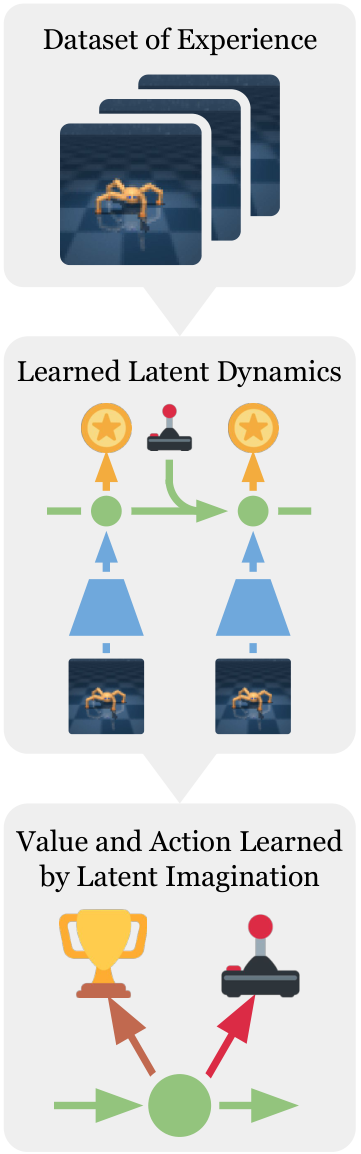
\includegraphics[width=0.95\linewidth,height=0.78\textheight,keepaspectratio]{assets/New-Lecture_World_Models/towardsai_primer_dreamer_hafner2020_iclr_p1_teaser.png}\\[0.12em]
        {\scriptsize Hafner et al., \href{https://arxiv.org/pdf/1912.01603.pdf}{\textit{Dream to Control}}. Chen, \href{https://pub.towardsai.net/dreamer-8b5a42acebbf}{Towards AI} (2020).}
      \end{column}
    \end{columns}
\end{frame}

\begin{frame}[t]{Dreamer: architecture}
  \centering
  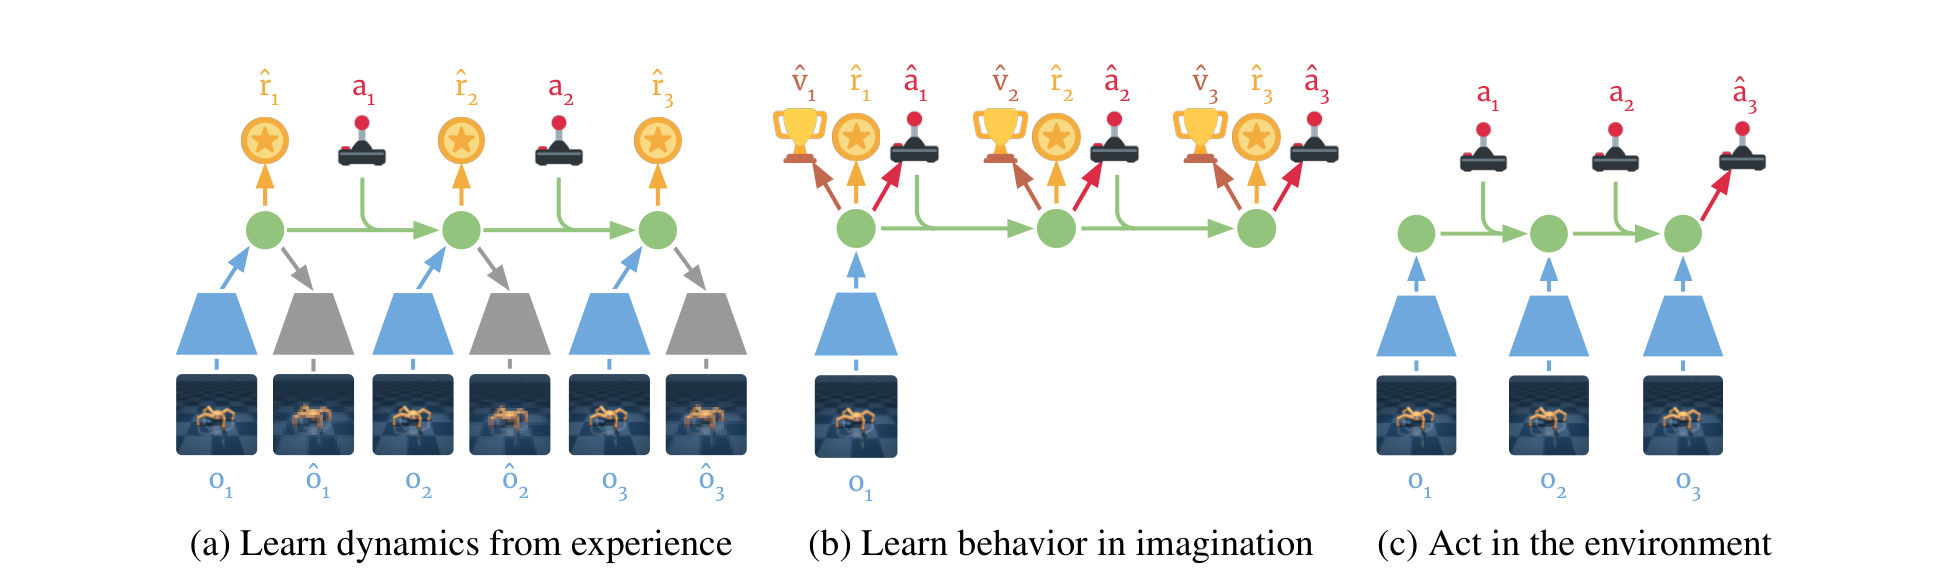
\includegraphics[width=\linewidth,height=0.84\textheight,keepaspectratio]{assets/New-Lecture_World_Models/towardsai_primer_dreamer_hafner2020_iclr_fig3_components.png}
  {\tiny Dreamer architecture. Diagram credit: Hafner et al.\ (ICLR 2020), \href{https://arxiv.org/pdf/1912.01603.pdf}{PDF}}  
  \break
  Dreamer is composed of three main parts: 
  \begin{itemize}\itemsep0.08em \footnotesize
    \item \textbf{ (a) Dynamics Learning:} learns representation, transition, reconstruction, reward models.
    \item \textbf{ (b) Behavior Learning:} based on the dynamics model, learns actor--critic architecture to maximize rewards.  
    \item \textbf{ (c) Environment Interaction:} using action model for data collection.
  \end{itemize}
\end{frame}

\begin{frame}[t]{DreamerV2: discrete world model \& V1 $\rightarrow$ V2}
  \begin{columns}
    \column{0.64\textwidth}
    \centering
    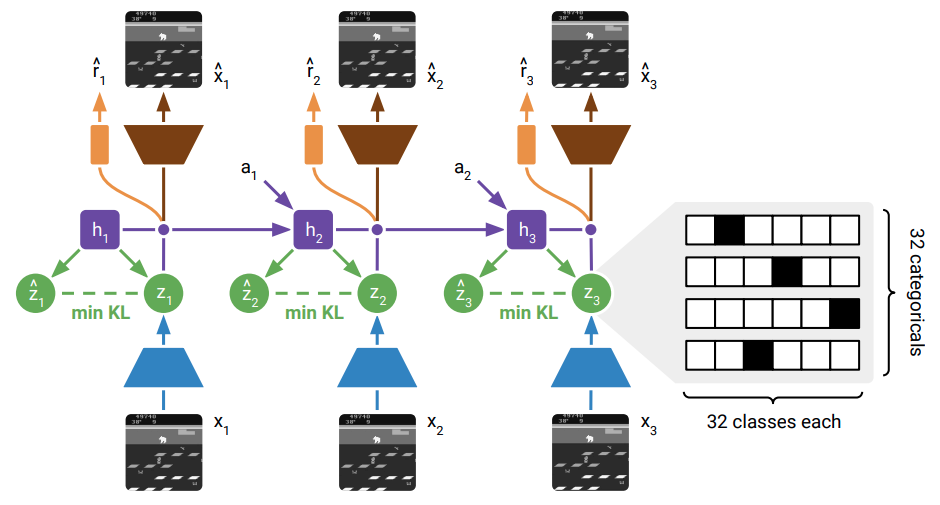
\includegraphics[width=0.94\linewidth,height=0.94\textheight,keepaspectratio]{assets/New-Lecture_World_Models/eclecticsheep_dreamerv2_worldmodel_arch.png}\\[0.08em]
    {\tiny World-model overview. Diagram credit: Belotti (2023)}
    \column{0.36\textwidth}
    \begin{itemize}\footnotesize
      \item \textbf{Key upgrade:} The world model now uses \textbf{discrete categorical latents} instead of continuous Gaussian variables. Each latent consists of 32 variables, each taking one of 32 categories, enabling a richer and more expressive latent space.
      \item Discrete latents are optimized using \textbf{straight-through gradients} for effective backpropagation despite non-differentiability. This allows for more precise representation and imagination.
      \item \textbf{KL balancing} is introduced to stabilize training by balancing the KL divergence term across model components.
    \end{itemize}
  \end{columns}
\end{frame} 

\begin{frame}[t]{DreamerV3: motivation}
  \begin{itemize}\itemsep0.10em
    \item Achieves state-of-the-art performance across 150+ diverse tasks with a single configuration.
    \item Learns a world model to imagine future trajectories. Successfully solves challenging open-world environments such as collecting diamonds in Minecraft without human data.
    \item Architecturally similar to DreamerV2. Robustness and scalability stem from careful normalization, balancing, and mathematical tricks that enable stability across domains.
  \end{itemize}
\end{frame}

\begin{frame}[t]{DreamerV3: architecture}
  Learning algorithm consists of three neural networks:
  \begin{itemize}\itemsep0.06em\footnotesize
    \item \textbf{World model:} RSSM model that predicts the outcomes of potential actions, modeling future states of the environment.
    \item \textbf{Critic:} Judges the value of each predicted outcome, estimating how beneficial a state is for achieving the agent's goals.
    \item \textbf{Actor:} Selects actions intended to achieve the most valuable outcomes by maximizing the evaluated value.
  \end{itemize}
  \vspace{-0.4em}
  \centering
  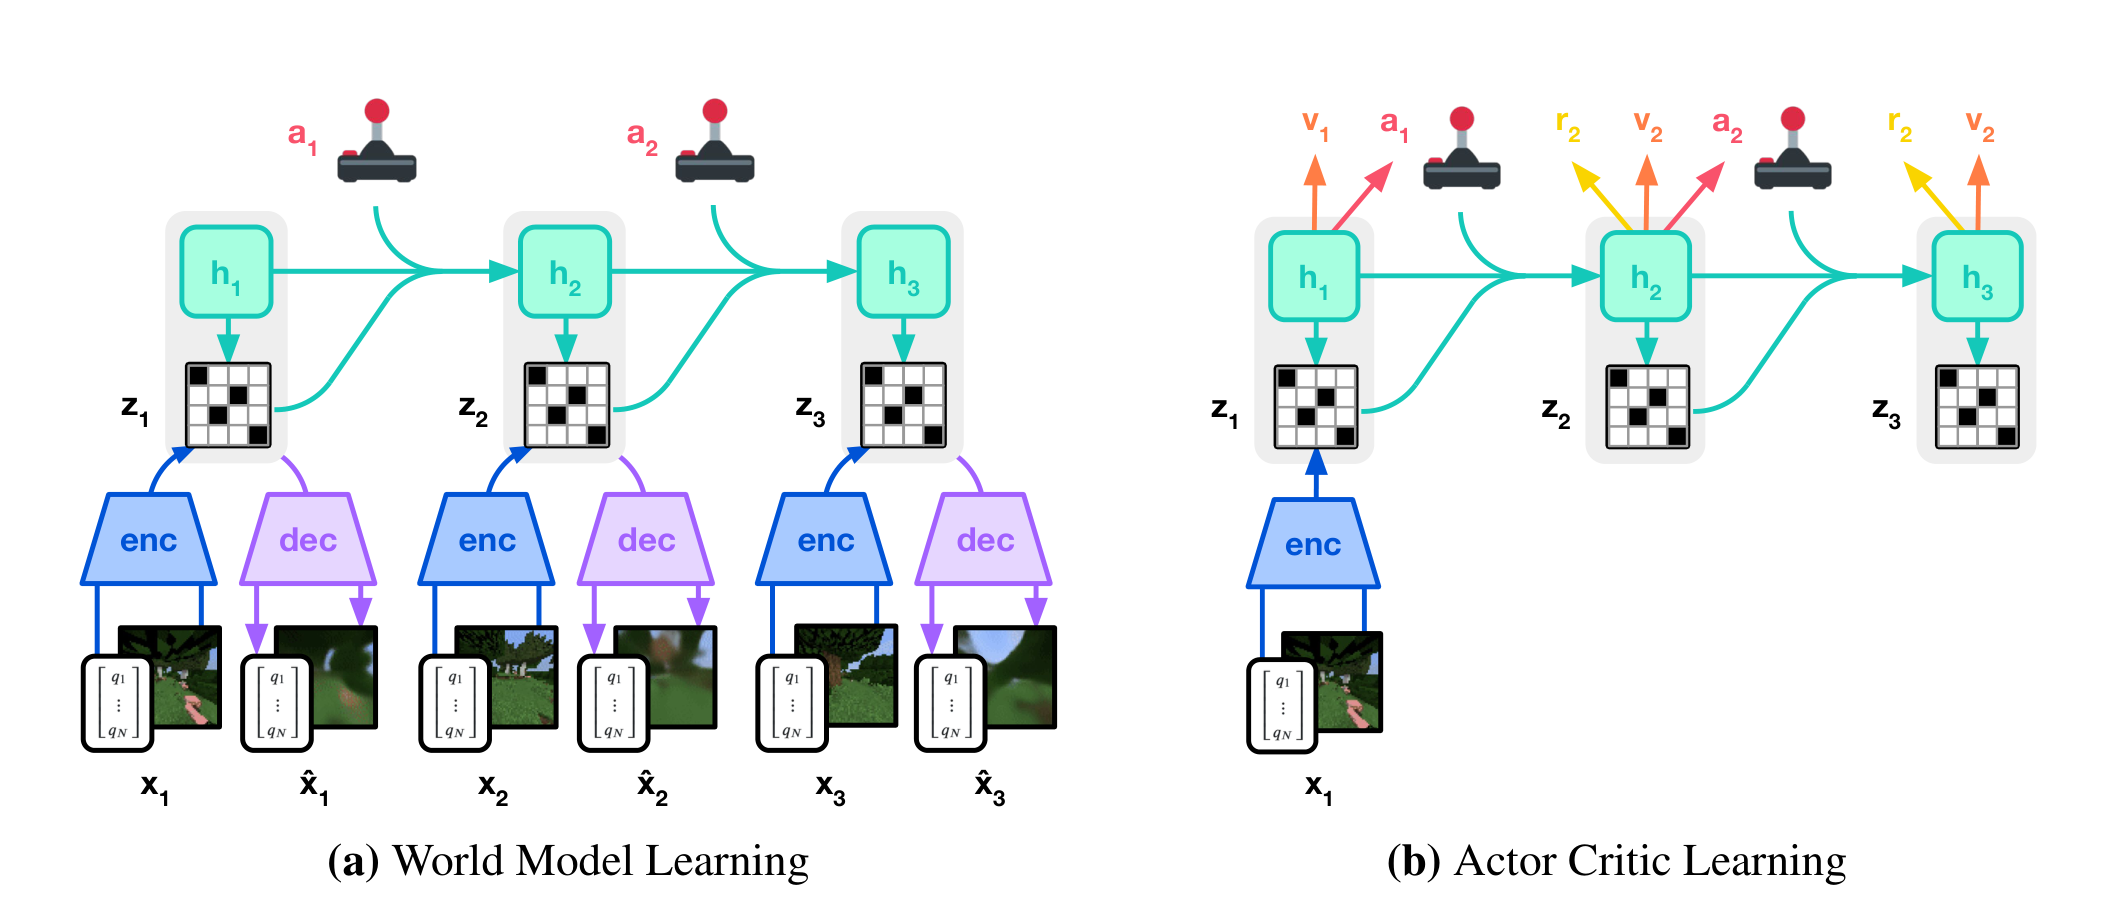
\includegraphics[width=\linewidth,height=0.46\textheight,keepaspectratio]{assets/New-Lecture_World_Models/dreamerv3_arxiv2301_fig3_training_process.png}\\[0.03em]
  {\scriptsize Hafner et al., \href{https://arxiv.org/pdf/2301.04104.pdf}{arXiv:2301.04104}.}
\end{frame}


% \begin{frame}[t]{DreamerV3: results}
%   \centering
%   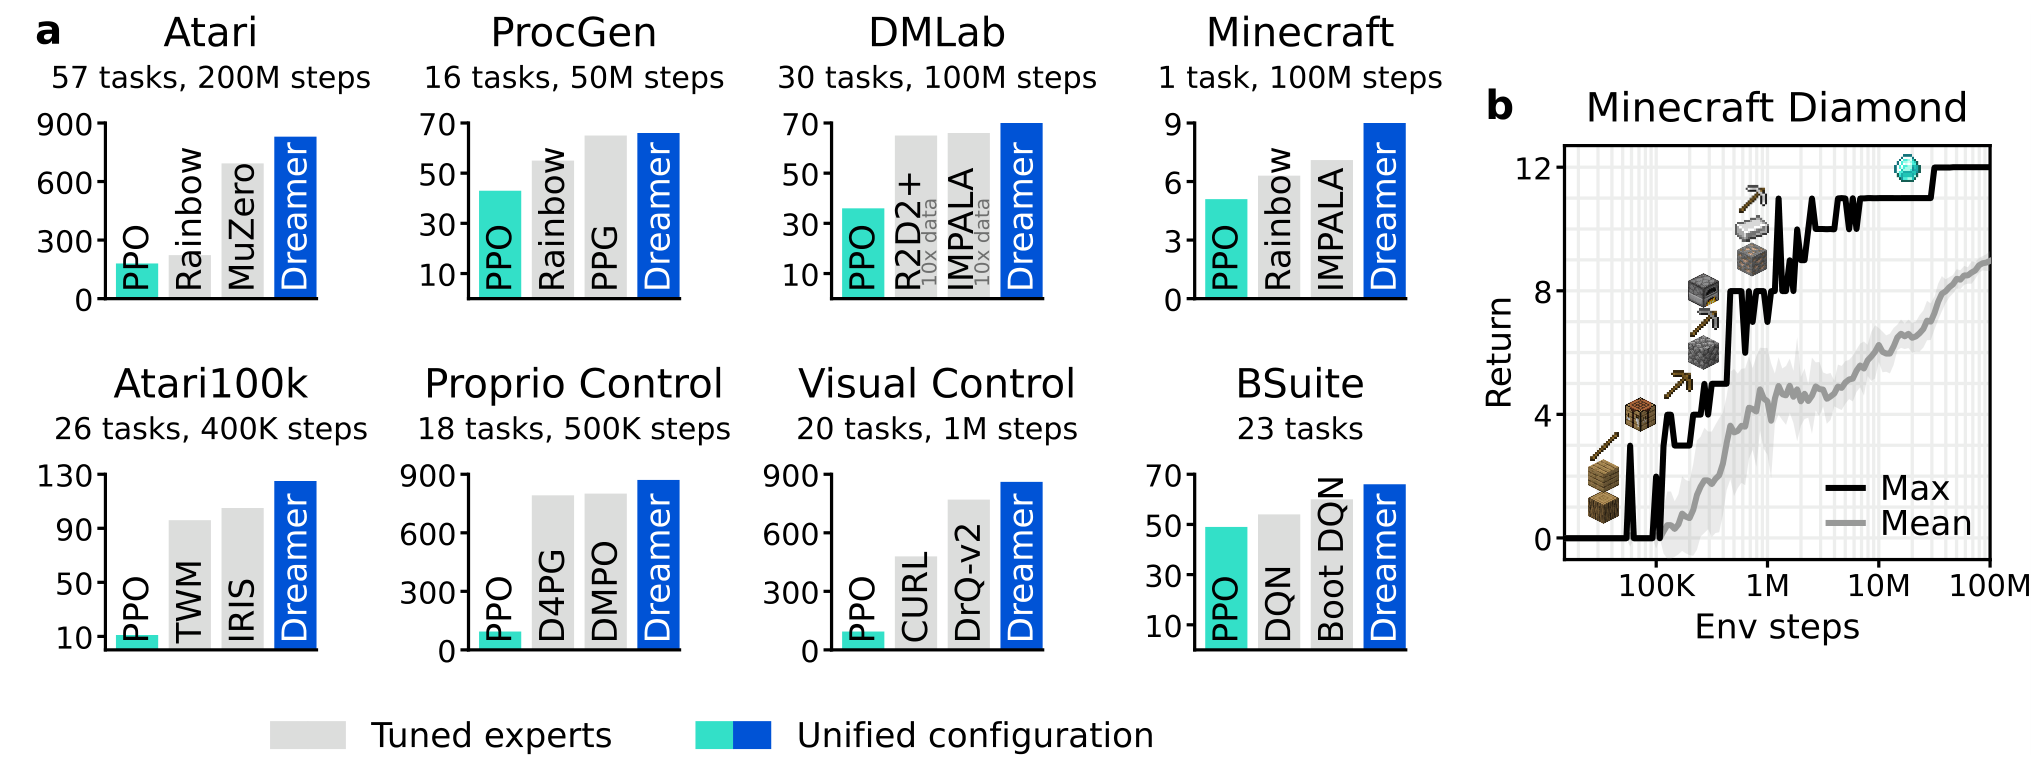
\includegraphics[width=\linewidth,height=0.78\textheight,keepaspectratio]{assets/New-Lecture_World_Models/dreamerv3_arxiv2301_fig1_benchmark_summary.png}\\[0.06em]
%   {\scriptsize Benchmark summary. a, Using fixed hyperparameters across all domains, Dreamer
%   outperforms tuned expert algorithms across a wide range of benchmarks and data budgets. Dreamer
%   also substantially outperforms a high-quality implementation of the widely applicable PPO algorithm.
%   b, Applied out of the box, Dreamer learns to obtain diamonds in the popular video game Minecraft
%   from scratch given sparse rewards, a long-standing challenge in artificial intelligence for which
%   previous approaches required human data or domain-specific heuristics. Hafner et al., \href{https://arxiv.org/pdf/2301.04104.pdf}{arXiv:2301.04104}.}
% \end{frame}
